\documentclass[tikz,convert={outfile=\jobname.svg}]{standalone}

\usetikzlibrary{shapes.misc}

\tikzset{cross/.style={cross out, draw=black, minimum size=2*(#1-\pgflinewidth), inner sep=0pt, outer sep=0pt},
%default radius will be 1pt. 
cross/.default={2.5pt}}

\begin{document}

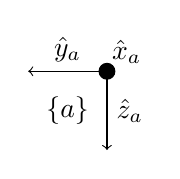
\begin{tikzpicture}
    \draw [->] (0,0) -- (-1, 0) node[pos=0.5, above]{$\hat{y}_{a}$};
    \draw [->] (0,0) -- (0, -1) node[pos=0.5, right]{$\hat{z}_{a}$};
    \filldraw (0,0) circle[radius=1mm]  node[pos=0, xshift=0.25cm, yshift=0.25 cm]{$\hat{x}_{a}$};
    \draw (0,0) node[pos=0, xshift=-0.5cm, yshift=-0.5cm]{$\{a\}$};
\end{tikzpicture}

\end{document}